
\documentclass{article}
 
\usepackage{amsmath}
\usepackage{amssymb}
\usepackage{graphicx}
\usepackage{verbatim}
\usepackage{enumerate}
\usepackage[utf8]{inputenc}
\newcommand{\beq}{\begin{equation}}
\newcommand{\eeq}{\end{equation}}
%\verbatiminput{verb.txt}
\begin{document}
\title{Project 1. FYS3150}
\author{Shafa Aria}
\maketitle
 
Introduction:
In this project we shall familiarize ourselves witht the various matrix operations, DMA and using the various libraries. The project itself evolves around Poisson equation and the numerical implementation of it using linear algebra packages for C++. We will in the following solve the linear equations and find numerical solutions for the equation and compare it with the analytical solution. This project was a collaboration with Abas Omar. 
 
\newpage
 
 
\begin{enumerate}
\item[(a)]
 
Our equation may be rewritten by multiplying with h squared:
\[
   2v_i - v_{i+1} - v_{i-1}= f_ih^2
\]
We recognise the RHS as given to us being $b_i = h^2f_i$ this is a simple difference equation that can be rewritten as the product of 2 matrices where {\bf A} contains the constant values and {\bf v} the function values.
 
\[
   2\cdot v_i - 1\cdot v_{i+1} - 1 \cdot v_{i-1}= f_i h^2
\]
 
\beq
    {\bf Av} = \left[\begin{array}{cccccc}
                           a_1& a_2& a_3 &\dots   & \dots &a_n \\
                       \end{array} \right]\left[\begin{array}{c}
                           v_1\\
                           v_2\\
                           v_3\\
                          \dots  \\
                          \dots \\
                           v_n\\
                      \end{array} \right]
\eeq
\beq
\hspace{1.05cm} = \hspace{0cm} \left[\begin{array}{c}
                           a_1\cdot v_1 +  a_2\cdot v_2  +a_3\cdot v_3 + \dots + a_n\cdot v_n\\
                      \end{array} \right]
\eeq
 
 
\item[(b)]
 
We realise that our matrix contains only three constants across the diagonal and thus we can write them as vectors instead of having the entire matrix written. We will then write an algorithm that will collect all the contributing factors.
 
\beq
    {\bf a} = \left[\begin{array}{c}
                           a_2\\
                           a_3\\
                           a_4\\
                          \dots  \\
                          \dots \\
                           a_n\\
                      \end{array} \right]
    {\bf b} = \left[\begin{array}{c}
                           b_1\\
                           b_2\\
                           b_3\\
                          \dots  \\
                          \dots \\
                           b_n\\
                      \end{array} \right]
    {\bf c} =\left[\begin{array}{c}
                           c_1\\
                           c_2\\
                           c_3\\
                          \dots  \\
                          \dots \\
                           c_{n-1}\\
                      \end{array} \right]
\eeq
 
We will use forward substitution to remove the lower diagonal and then backward substition to remove the upper diagonal.
For the forward we find:
 
 
\[
    \tilde{b}_{i+1}= \tilde{b}_{i+1} - \tilde{b}_{i}\frac{ a_{i+1}}{b_{i}} \hspace{0.5cm} \mathrm{for} \hspace{0.1cm} i=1,\dots, n-1
\]\[
     b_{i+1}=b_{i+1}-\frac{ a_{i+1}\cdot c_{i}}{b_{i}}  \hspace{0.5cm} \mathrm{for} \hspace{0.1cm} i=1,\dots, n-1
\]
And for the backwards:
\[
     \tilde{b}_{i-1}=\tilde{b}_{i-1}-c_{i-1}\cdot \frac{\tilde{b}_i}{b_i} \hspace{0.5cm} \mathrm{for} \hspace{0.1cm} i=n,\dots, 1
\]
And thus:
\[
x_i= \frac{\tilde{b}_i}{b_i}
\]
For total FLOP we count our iterations: $2\cdot(3\cdot (n-1))$ for forward,$3n+n$ for backwards. Total of $10n-6$ FLOP and arithmetic complexity of $O(n^2)$ for this algorithm. For comparison LU and Gaussian Elimination requires $2/3 n^3$ has arithmetic complexity of $O(n^3)$.
 
\hspace{-0.4cm}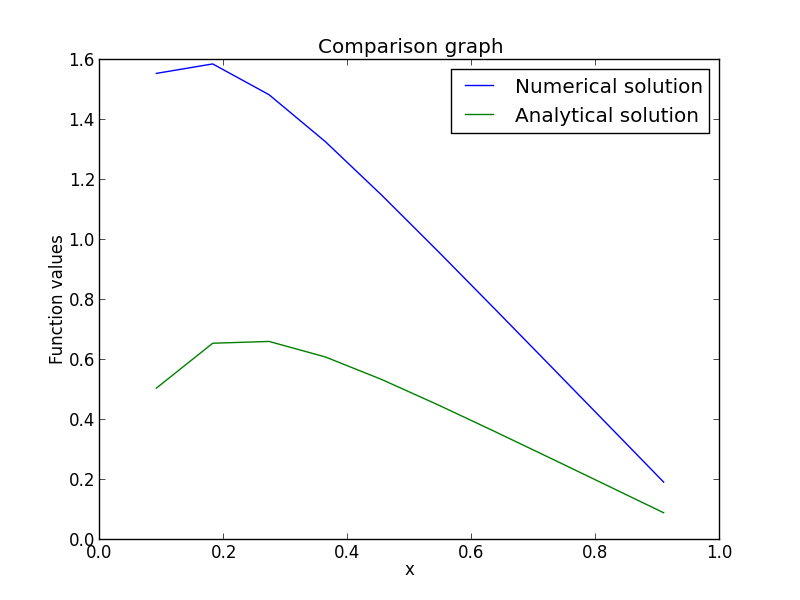
\includegraphics[scale=0.3]{P10x.png}\hspace{0.1cm} 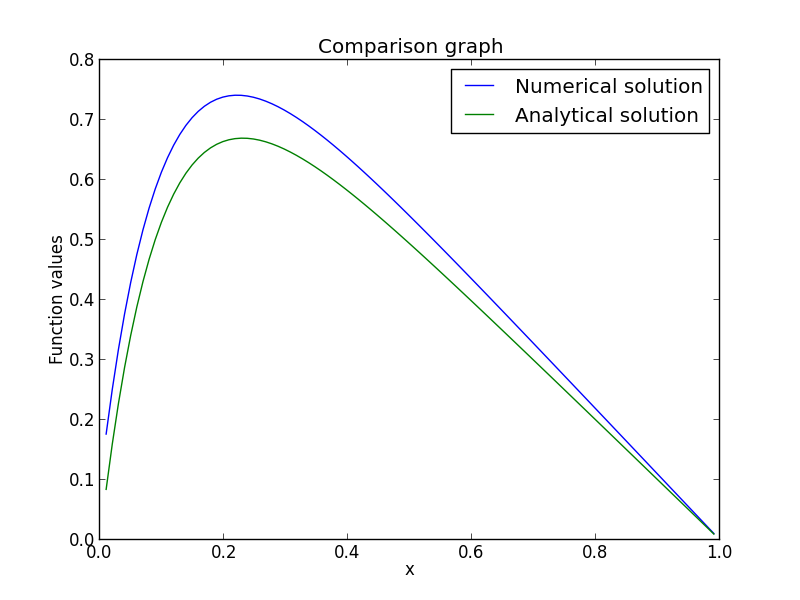
\includegraphics[scale=0.3]{P100x.png}\\
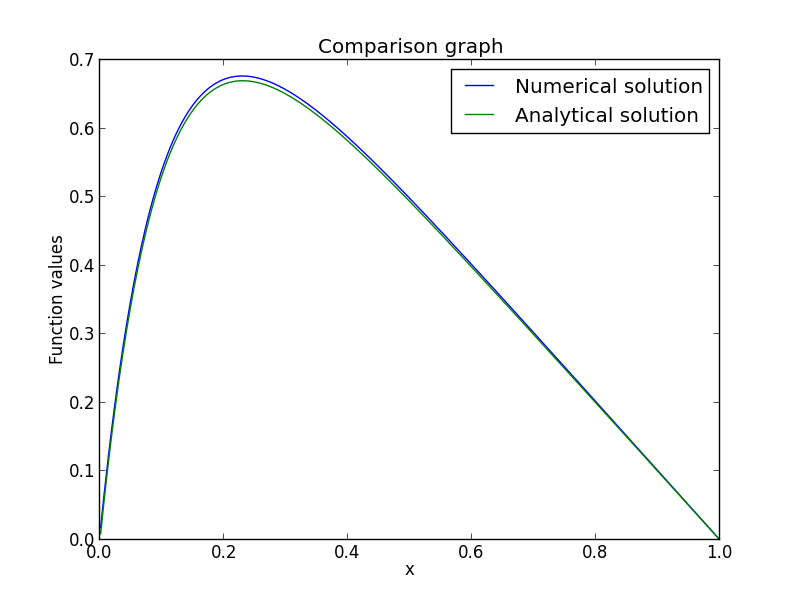
\includegraphics[scale=0.4]{P1000x.png}\\
 
As we can see shorter steps gives higher accuracy, and thus our numerical calculation approximates the analytical solution better. From top left: $n=10$, $n=100$ and at the bottom $n=1000$. Albeit as we can see despite $n=1000$ we can clear see there's a difference between the two, but as we shorten our step the curve lies more and more onto the analytical one. 
%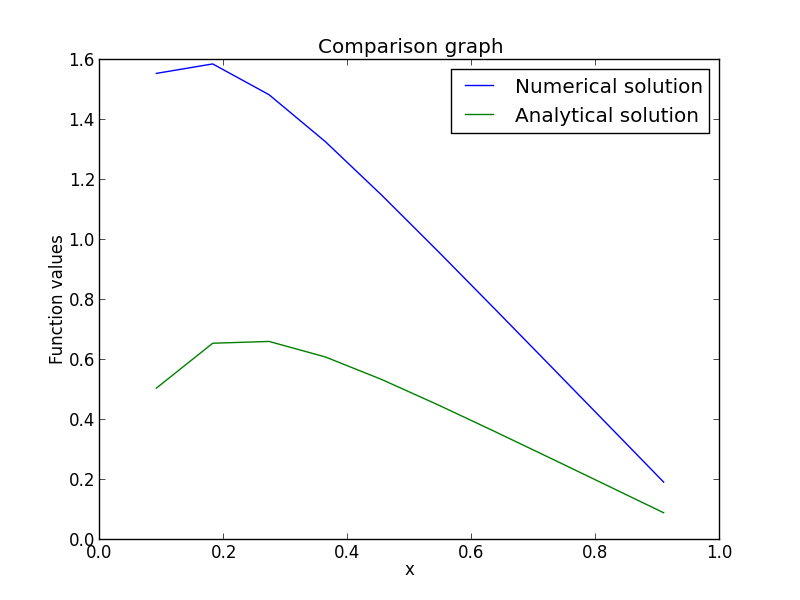
\includegraphics[scale=0.5]{P10x.png}\\
 
\item[(c)]
The expected results is of course that the accuracy will increase, but we see that the relative error is approximately porportional to the log(h). The order of the relative error is therefore approximately the same as h.
\beq
\left[\begin{array}{cc}
                          \mathrm{log(h) = -1} & \mathrm{epsi=0.728827503126}\\
                          \mathrm{log(h) = -2} & \mathrm{epsi=0.088645078904}\\
                          \mathrm{log(h) = -3} & \mathrm{epsi=0.009085353860}\\
                          \mathrm{log(h) = -4} & \mathrm{epsi=0.000910799789}\\
                          \mathrm{log(h) = -5} & \mathrm{epsi=9.11346953e-05}\\
                      \end{array} \right]
\eeq
\newpage
\item[(d)]
As for d we are supposed to compare our results with the LU decomposition for the various steps and see how long the computation takes. As it is now we could not get our code to work, there's a mismatch between the armadillo package and the vector/matrix opreations. Albeit the code is included. 

\item[(e)]
See the code.


Comment: the link for the github: 

https://github.com/Ace-/Project-1
\end{enumerate}
%\verbatiminput{opp11.m}
%\includegraphics[scale=0.5]{oppg7.png}\\
%\begin{align*}
%\hspace{2cm} &
%\end{align*}
%\pagebreak
\end{document}

